%==============================================================================
%  CHAPITRE 1 — FONDEMENTS
%==============================================================================
\titreduchapitre{Fondements de l'apprentissage adaptatif et de l'engagement}{chap:fondements}

%==============================================================================
\section{Introduction}
\label{sec:fond-intro}

La conception d'un système d'apprentissage adaptatif fondé sur
l'engagement émotionnel mobilise un ensemble de notions issues de
domaines distincts : sciences de l'éducation, informatique affective,
apprentissage multimodal et intelligence artificielle générative. Ces
notions sont souvent présentées séparément ; les rassembler permet
d'établir un vocabulaire partagé et d'expliciter les hypothèses sur
lesquelles repose le pipeline \emolearn{}.

Ce chapitre examine les concepts fondamentaux nécessaires à la
compréhension de cette architecture. Il aborde successivement
l'apprentissage en ligne et les MOOC, la notion d'engagement de
l'apprenant, les apports de l'informatique affective, les principes de
la détection multimodale, puis les bases de l'intelligence artificielle
générative appliquée à l'éducation (LLM, guidage par prompts et RAG).

%==============================================================================
\section{Apprentissage en ligne et MOOC}
\label{sec:fond-mooc}

\subsection{Définition}

Les cours en ligne ouverts et massifs (MOOC, \emph{Massive Open Online
Courses}) désignent des dispositifs de formation accessibles à distance, le
plus souvent sans prérequis d'inscription stricts, et destinés à un public
potentiellement très large \cite{daniel2012making,breslow2013studying}. Ils
reposent typiquement sur des vidéos pédagogiques, des quiz, des forums et un
parcours de progression asynchrone.

\subsection{Implication pour l'adaptation}

Dans ce modèle, le contenu est principalement diffusé de manière uniforme.
Toute forme d'adaptation automatique suppose donc, en amont, de disposer
d'une mesure d'engagement plus fine que les simples proxies de présence
(connexion, clics), point développé dans la section suivante.

%==============================================================================
\section{Engagement de l'apprenant}
\label{sec:fond-engagement}

\subsection{Définition}

L'engagement désigne la mobilisation cognitive, comportementale et
émotionnelle de l'apprenant vis-à-vis de la tâche d'apprentissage
\cite{kizilcec2013deconstructing,hew2016promoting,fredricks2004school}. Il ne se réduit pas à la
simple présence en ligne (connexion, clics), mais renvoie à une implication
active dans le traitement de l'information.

\subsection{Dimensions de l'engagement}

On distingue classiquement :


\begin{figure}[H]
\centering
\begin{tikzpicture}[
  box/.style={rectangle, rounded corners=3pt, draw=#1, thick, fill=#1!12,
              minimum width=3.6cm, minimum height=1.55cm, align=center,
              font=\small},
  arr/.style={-{Stealth[length=2.4mm]}, thick, gray!70}
]
\node[box=teal!70!black] (cog) {\textbf{Cognitif}\\profondeur du traitement\\stratégies d'apprentissage};
\node[box=blue!70!black, right=0.55cm of cog] (beh) {\textbf{Comportemental}\\participation\\persévérance};
\node[box=orange!80!black, right=0.55cm of beh] (emo) {\textbf{Émotionnel}\\intérêt, ennui,\\frustration, etc.};
\node[draw=gray!55, dashed, rounded corners=4pt, fit=(cog)(beh)(emo),
      inner sep=8pt, label={[font=\small\bfseries]above:Engagement de l'apprenant}] {};
\node[below=0.35cm of emo, font=\footnotesize\itshape, text=orange!80!black, align=center]
  {Focus \emolearn{}};
\end{tikzpicture}
\caption{Les trois dimensions classiques de l'engagement. }
\label{fig:fond-dimensions-engagement}
\end{figure}

\emolearn{} se concentre principalement sur la dimension émotionnelle /
affective, tout en visant un effet sur la persévérance globale.

\subsection{Mesure de l'engagement}

Les indicateurs usuels en e-learning (durée de session, progression, scores)
fournissent des \emph{proxies} utiles mais incomplets. Les approches plus
récentes mobilisent des signaux multimodaux (visage, voix, posture) pour
estimer l'état affectif de manière plus directe
\cite{dmello2015review,sharma2020multimodal,goldberg2021attentive}.

%==============================================================================
\section{Informatique affective et émotions en apprentissage}
\label{sec:fond-affect}

\subsection{Rôle des émotions dans l'apprentissage}

Les travaux en psychologie de l'apprentissage montrent que les émotions
modulent l'attention, la mémorisation et la persévérance
\cite{pekrun2006control,dmello2012dynamics,baker2010better,loderer2020beyond,graesser2020emotions}. Elles ne sont
donc pas périphériques à la cognition, mais constitutives du processus
d'apprentissage.

\subsection{États pertinents pour l'adaptation pédagogique}

Dans le cadre de ce mémoire, quatre états issus du corpus \textsc{DAiSEE}
\cite{gupta2016daisee} structurent la taxonomie d'engagement :


\begin{figure}[H]
\centering
\begin{tikzpicture}[
  etat/.style={rectangle, rounded corners=3pt, draw=#1, very thick, fill=#1!14,
               minimum width=3.5cm, minimum height=1.7cm, align=center, font=\small},
  arr/.style={-{Stealth[length=2.4mm]}, thick, gray!65}
]
\node[etat=green!55!black] (eng) {\textbf{Engagement}\\implication positive\\maintenir / enrichir};
\node[etat=gray!70!black, right=0.7cm of eng] (bor) {\textbf{Ennui}\\sous-stimulation\\relancer};
\node[etat=blue!65!black, below=0.65cm of eng] (con) {\textbf{Confusion}\\incompréhension\\clarifier};
\node[etat=red!65!black, right=0.7cm of con] (fru) {\textbf{Frustration}\\blocage\\soutenir / simplifier};
\node[draw=black!40, rounded corners=5pt, fit=(eng)(bor)(con)(fru),
      inner sep=10pt,
      label={[font=\small\bfseries]above:Taxonomie \textsc{DAiSEE} (4 états)}] {};
\end{tikzpicture}
\caption{Taxonomie des quatre états d'engagement retenus (\textsc{DAiSEE}).}
\label{fig:fond-taxonomie-daisee}
\end{figure}

Chacun de ces états appelle une stratégie pédagogique distincte.

\subsection{Charge cognitive}

La théorie de la charge cognitive rappelle qu'un contenu trop dense ou mal
séquencé favorise la confusion et l'abandon
\cite{sweller1988cognitive,sweller2019cognitive}. La théorie de
l'apprentissage multimédia complète ce cadre : la conception des messages
(texte, image, rythme) conditionne la charge utile
\cite{mayer2021multimedia}. L'adaptation du niveau d'explication, du rythme
et du type d'exemple constitue dès lors un levier central des systèmes
d'apprentissage adaptatifs.

%==============================================================================
\section{Détection multimodale de l'engagement}
\label{sec:fond-detection}

\subsection{Modalités exploitées}

La détection automatique de l'engagement peut s'appuyer sur :
\begin{itemize}
  \item le \textbf{visage} (expressions faciales, regard)~;
  \item la \textbf{voix} (prosodie, intensité, variations émotionnelles)~;
  \item éventuellement la posture ou des signaux physiologiques.
\end{itemize}
\emolearn{} combine les deux premières modalités, à partir de clips
vidéo et audio annotés (hors temps réel), plutôt que de traces textuelles
de forums ou de capteurs physiologiques.

\begin{figure}[H]
\centering
\begin{tikzpicture}[
  box/.style={rectangle, rounded corners=3pt, draw=black!70, thick,
              minimum width=2.5cm, minimum height=1.05cm, align=center, font=\small},
  io/.style={rectangle, rounded corners=2pt, draw=black!50, dashed,
             minimum width=2.4cm, minimum height=0.9cm, align=center, font=\footnotesize},
  arr/.style={-{Stealth[length=2.5mm]}, very thick, black!65}
]
\node[io] (vid) at (0,3.6) {Vidéo\\visage};
\node[io] (aud) at (4.2,3.6) {Audio\\voix};
\node[box, fill=blue!10] (fer) at (0,2.2) {FER};
\node[box, fill=blue!10] (ser) at (4.2,2.2) {SER};
\node[box, fill=teal!15] (fus) at (2.1,0.85) {Fusion\\multimodale};
\node[box, fill=orange!12] (etat) at (2.1,-0.55) {État\\d'engagement};
\node[box, fill=yellow!18] (adap) at (2.1,-1.95) {Adaptation\\pédagogique};

\draw[arr] (vid) -- (fer);
\draw[arr] (aud) -- (ser);
\draw[arr] (fer) -- (fus);
\draw[arr] (ser) -- (fus);
\draw[arr] (fus) -- (etat);
\draw[arr] (etat) -- (adap);
\end{tikzpicture}
\caption{Boucle conceptuelle de détection multimodale.}
\label{fig:fond-boucle-multimodale}
\end{figure}

\subsection{Corpus de référence}

Deux corpus publics fondent la chaîne de perception :
\begin{itemize}
  \item \textsc{DAiSEE} \cite{gupta2016daisee} pour l'engagement facial annoté~;
  \item \textsc{IEMOCAP} \cite{busso2008iemocap} pour l'émotion vocale et, via
  un sous-corpus audiovisuel, la validation de la fusion alignée.
\end{itemize}

\subsection{Fusion multimodale}

La fusion vise à combiner des sources hétérogènes pour obtenir une décision
plus robuste qu'une modalité seule
\cite{liang2024foundations,gandhi2023multimodal}. Elle soulève toutefois des
questions de pondération, de désaccord inter-modalités et de déséquilibre des
classes, qui seront traités dans la conception et la validation du système.

%==============================================================================
\section{IA générative pour l'éducation}
\label{sec:fond-ia}

\subsection{Grands modèles de langue}

Les grands modèles de langue (LLM, \emph{Large Language Models}) sont des
réseaux de neurones entraînés à prédire le prochain token d'une séquence à
partir d'un très grand corpus textuel
\cite{brown2020language,vaswani2017attention,wolf2020transformers,openai2023gpt4,dubey2024llama3}. Architecturée autour du
\emph{Transformer} décodeur, cette famille de modèles suit un pipeline
strictement séquentiel (figure~\ref{fig:fond-llm-arch}) : le texte d'entrée
est d'abord \emph{tokenisé} (mots ou sous-mots convertis en identifiants
numériques), puis ces identifiants passent dans une couche d'\emph{embeddings}
combinée à un encodage de position, avant d'entrer dans une pile de blocs
d'\emph{attention} et de couches \emph{feed-forward}. Une tête de langage
produit enfin la distribution sur le vocabulaire. La génération est
\emph{auto-régressive} : chaque token prédit est réinjecté pour produire le
suivant.

\begin{figure}[H]
\centering
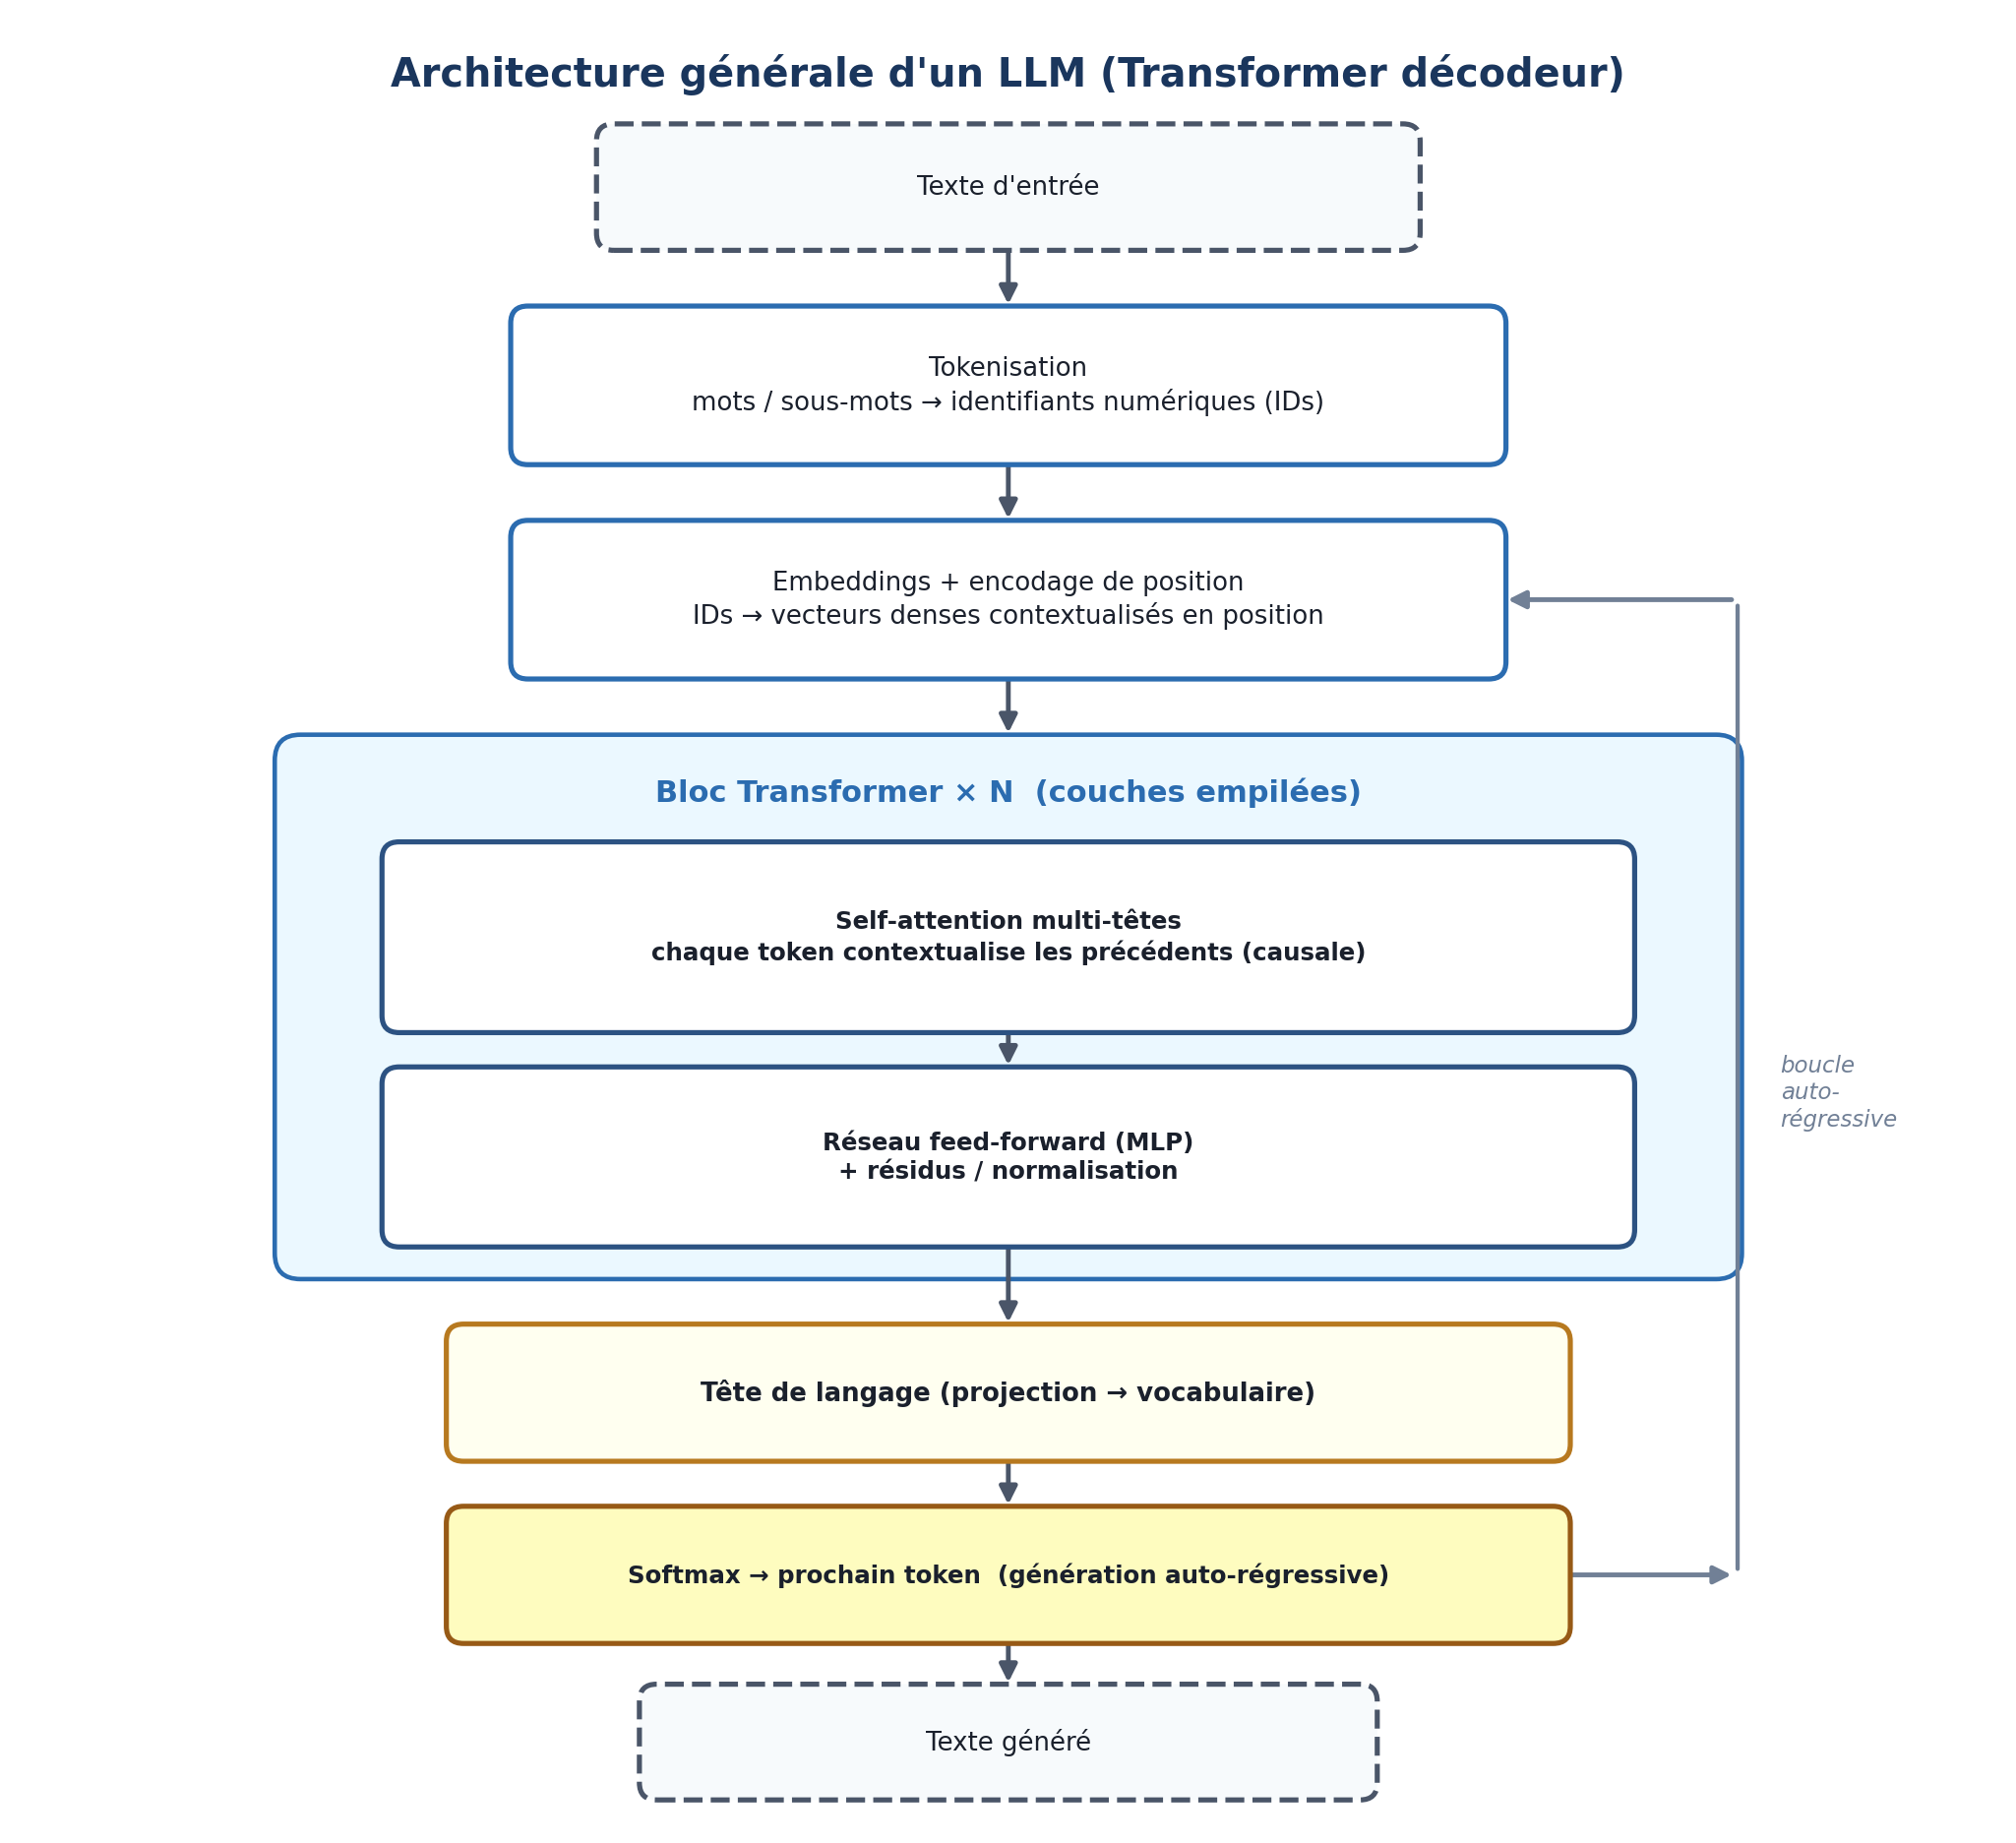
\includegraphics[width=0.88\textwidth]{figures/llm_architecture_generale.png}
\caption{Architecture générale d'un LLM de type Transformer décodeur.
}
\label{fig:fond-llm-arch}
\end{figure}

En éducation, ces modèles permettent de générer, à la demande, des
explications, reformulations, analogies ou encouragements en langage naturel
\cite{kasneci2023chatgpt,lo2023chatgpt,yan2024practical,wang2024large}. Ils offrent ainsi une voie crédible pour produire
des contenus pédagogiques personnalisés à grande échelle.

\subsection{Guidage par prompts et patrons}

La qualité du contenu généré dépend fortement du guidage
\cite{liu2023pretrain,white2023prompt,wei2022chain}. Une bibliothèque de
patrons de prompts structurés permet de conditionner la génération selon
l'état d'engagement détecté et le type d'intervention pédagogique souhaité.

\subsection{Récupération augmentée (RAG)}

Le mécanisme de \emph{Retrieval-Augmented Generation} (RAG)
\cite{lewis2020retrieval,gao2023retrieval,fan2024survey} ancre la génération sur des documents de référence
indexés dans une base vectorielle (figure~\ref{fig:fond-rag}). Les documents
sont d'abord découpés et vectorisés (indexation hors ligne). À l'exécution,
la question est embedée puis confrontée à l'index pour récupérer les
passages les plus pertinents ; ces passages enrichissent le prompt transmis
au LLM, qui produit une réponse ancrée. Ce dispositif réduit le risque
d'hallucinations factuelles et renforce la cohérence pédagogique des
contenus produits.

\begin{figure}[H]
\centering
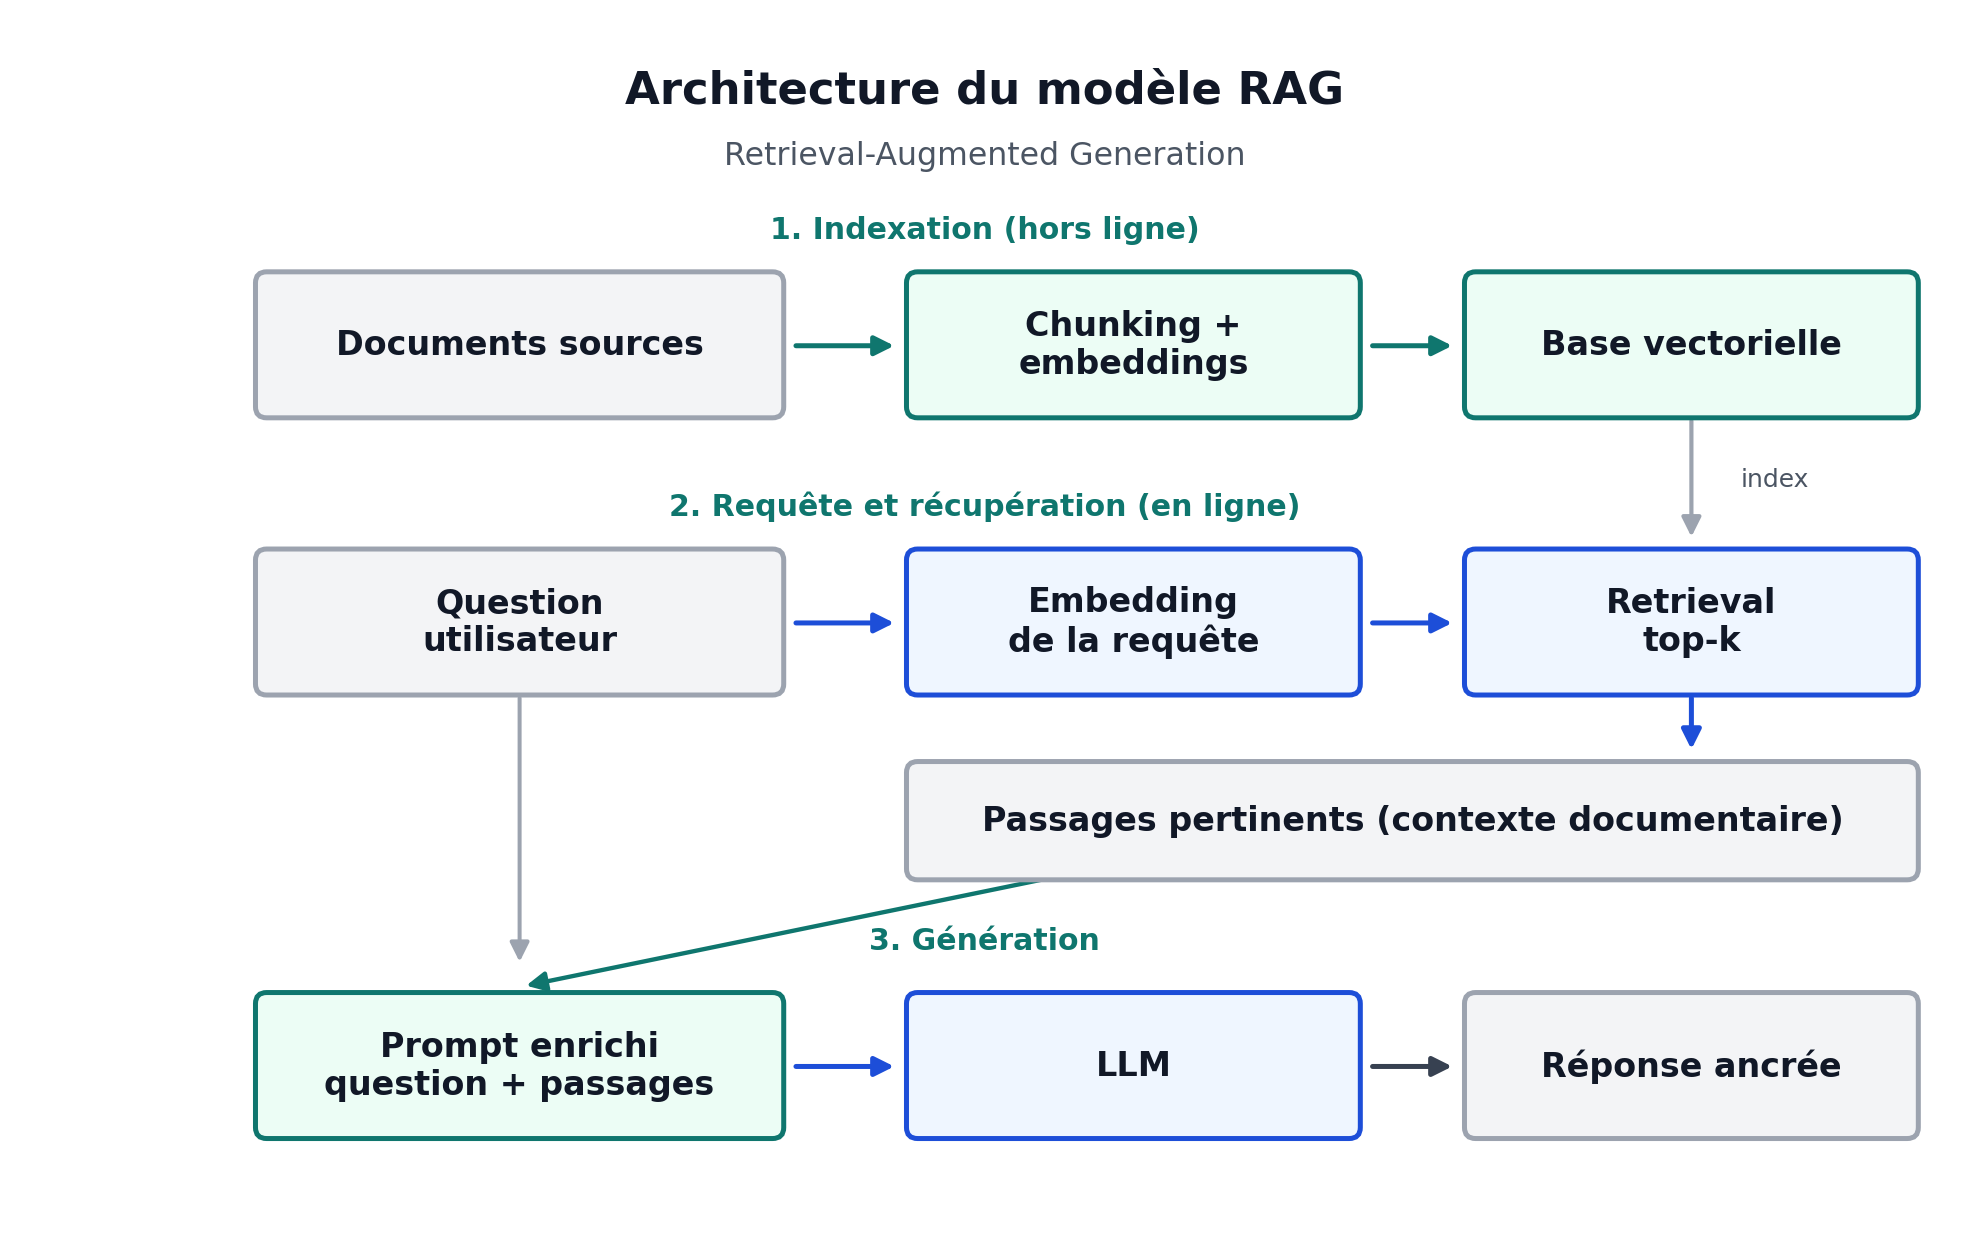
\includegraphics[width=0.92\textwidth]{figures/rag_architecture_generale.png}
\caption{Architecture générale du RAG.}
\label{fig:fond-rag}
\end{figure}

%==============================================================================
\section{Conclusion}
\label{sec:fond-concl}

Ce chapitre a rappelé le socle conceptuel sur lequel s'appuie \emolearn{} :
la définition des MOOC et l'enjeu d'adaptation, la centralité de
l'engagement émotionnel, les bases de la détection multimodale et le potentiel
de l'IA générative guidée et ancrée documentairement. Le chapitre suivant
examine l'état de l'art correspondant et positionne le présent travail par
rapport aux approches existantes.
